% 建议使用 XeLaTeX 或 LuaLaTeX 编译(更佳的中文支持)
\documentclass[UTF8,zihao=-4]{ctexart}

% 统一导言
\usepackage[a4paper,margin=2.5cm]{geometry}
\usepackage{amsmath,amssymb,amsthm}
\usepackage{bm}
\usepackage{hyperref}
\usepackage{graphicx}
\usepackage{caption}
\usepackage{listings}
\usepackage{xcolor}
\usepackage{float}
\usepackage{placeins}

% 图片路径
\graphicspath{{figures/}}

% 统一代码风格
\lstdefinestyle{code}{%
  language=Python,
  basicstyle=\ttfamily\small,
  numbers=left,
  numberstyle=\tiny, 
  keywordstyle=\color{blue}\bfseries,
  commentstyle=\color{teal!70!black},
  stringstyle=\color{orange!70!black},
  breaklines=true,
  frame=single,
  rulecolor=\color{black!30},
  tabsize=2,
  showstringspaces=false
}
\lstset{style=code}

\title{决策树:理论与实践}
\author{}
\date{\today}

\begin{document}
\maketitle
\tableofcontents

% 结构:Introduction / Theory and Formulas / Applications and Tips / Python Practice / Result / Summary

\section{引言}
决策树(Decision Tree)通过递归划分特征空间,形成分段常数的预测模型。其优点是可解释性强、对数据预处理要求低,并能处理非线性边界。

\section{原理与公式}
以分类树为例,在每个节点选择能够最大化“纯度提升”的划分。设节点数据集为 $\mathcal{D}$,类别占比为 $p_k$。常见纯度指标有基尼与熵:
\begin{align}
\mathrm{Gini}(\mathcal{D}) &= 1 - \sum_k p_k^2,\\
\mathrm{Entropy}(\mathcal{D}) &= -\sum_k p_k \log p_k.
\end{align}
若划分为左右子节点 $L,R$,则划分后的纯度为
\begin{equation}
I_{\mathrm{split}} = \frac{|L|}{|\mathcal{D}|} I(L) + \frac{|R|}{|\mathcal{D}|} I(R),
\end{equation}
最优划分使得 $\Delta I = I(\mathcal{D}) - I_{\mathrm{split}}$ 最大。停止条件常包括:最大深度、叶子最小样本数、最小纯度提升等。

\section{应用与技巧}
\begin{itemize}
  \item \textbf{优点:} 可解释、能处理非线性、对特征尺度不敏感、可处理类别与数值特征(需编码)。
  \item \textbf{缺点:} 容易过拟合、方差较大;可用集成方法缓解。
  \item \textbf{正则化:} 调整 \texttt{max\_depth}、\texttt{min\_samples\_leaf},或使用复杂度剪枝。
  \item \textbf{基线对比:} 与逻辑回归、SVM、随机森林等模型对比评估。
\end{itemize}

\section{Python 实战}
在本章节目录运行下述命令,图片将保存到本目录的 \texttt{figures/}:
\begin{lstlisting}[style=code,caption={生成决策树配图},label={lst:genfigs_dt_cn}]
python gen_decision_tree_figures.py
\end{lstlisting}

% 将完整 Python 源码纳入文章
\lstinputlisting[style=code,caption={gen\_decision\_tree\_figures.py 源码},label={lst:source_dt_cn}]{gen_decision_tree_figures.py}

\section{结果}
\begin{figure}[H]
  \centering
  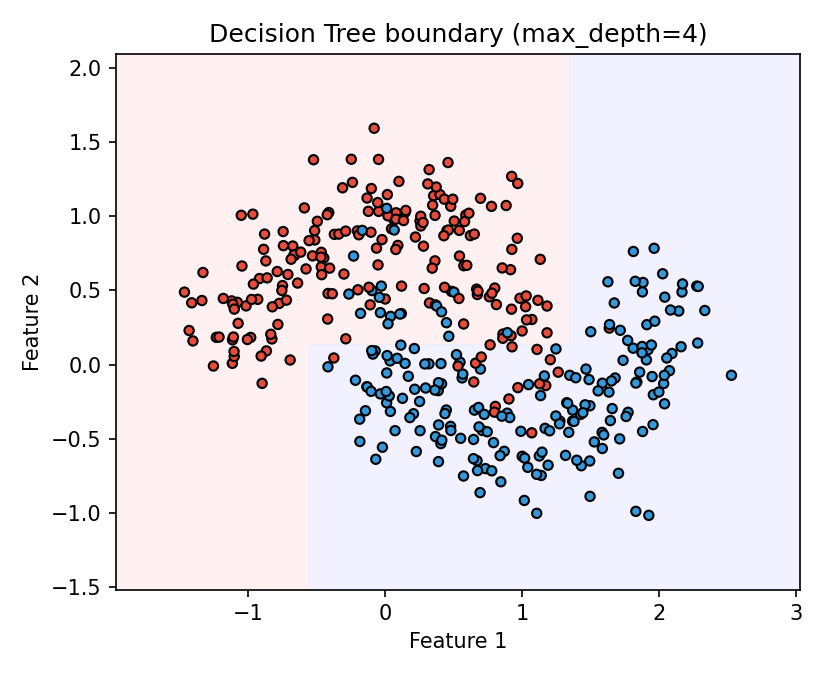
\includegraphics[width=0.9\linewidth]{dt_decision_boundary_2class.png}
  \caption{决策树在两类数据上的决策边界。}
  \label{fig:dt2_cn}
\end{figure}
\FloatBarrier

\begin{figure}[H]
  \centering
  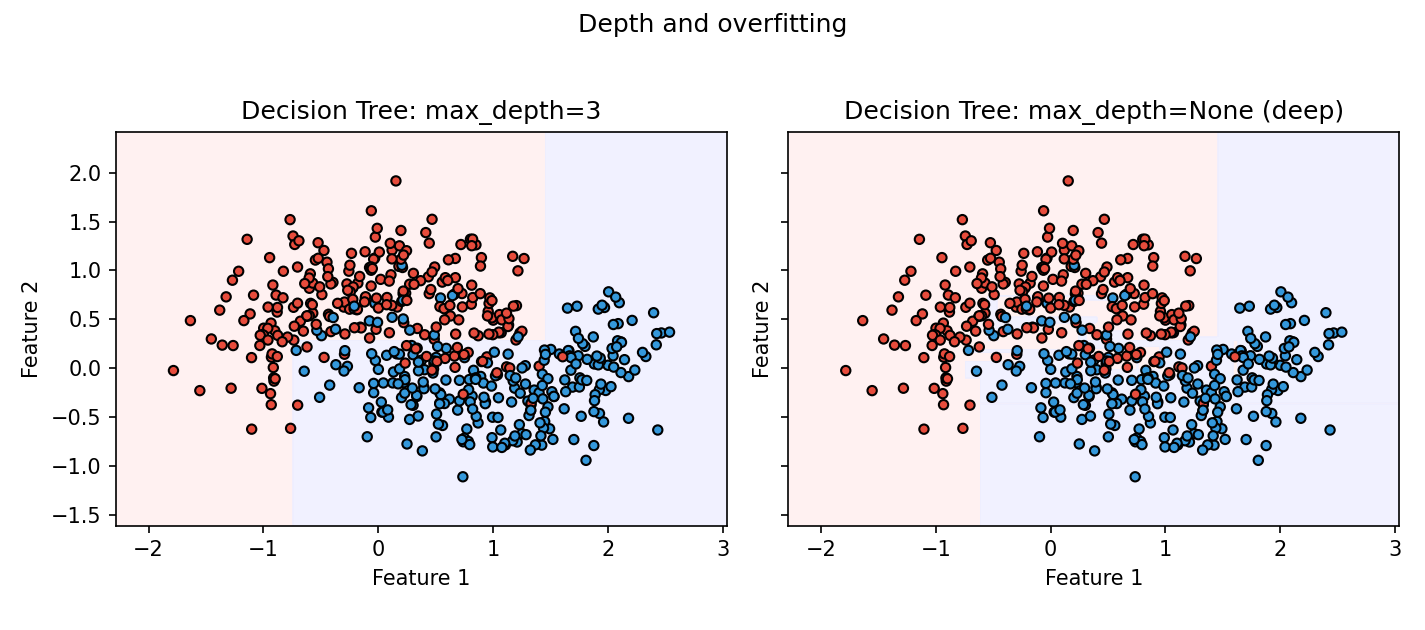
\includegraphics[width=0.95\linewidth]{dt_depth_compare.png}
  \caption{树深度影响:浅层与深层(过拟合)对比。}
  \label{fig:depth_cn}
\end{figure}
\FloatBarrier

\begin{figure}[H]
  \centering
  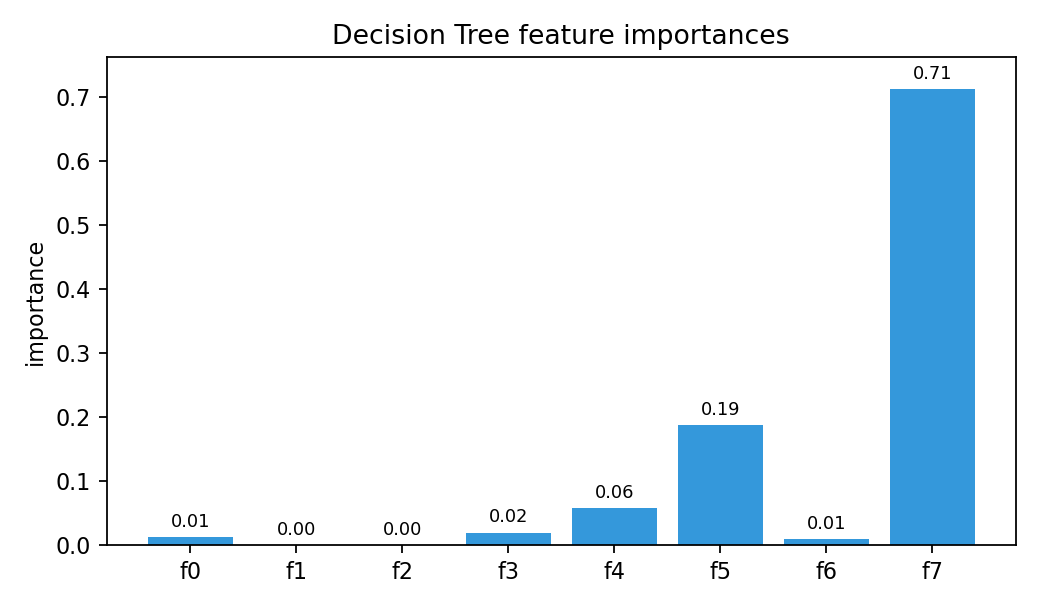
\includegraphics[width=0.85\linewidth]{dt_feature_importances.png}
  \caption{决策树的特征重要性可视化。}
  \label{fig:fi_cn}
\end{figure}
\FloatBarrier

\begin{figure}[H]
  \centering
  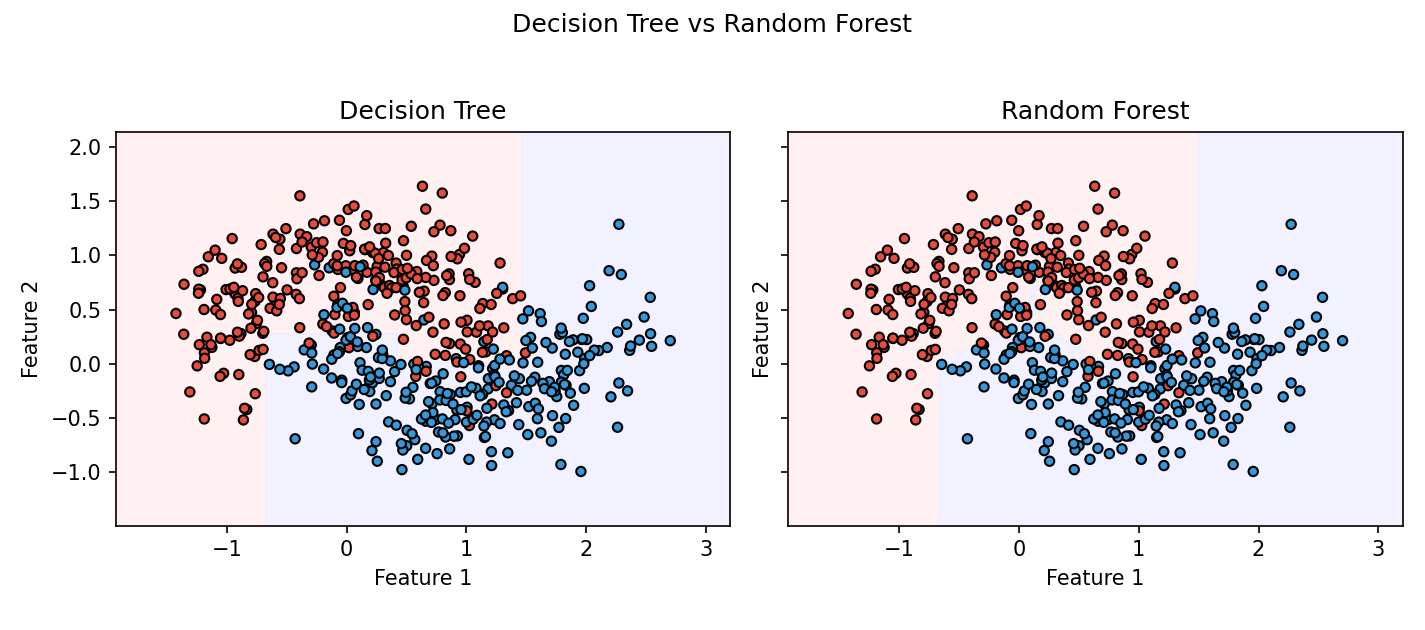
\includegraphics[width=0.95\linewidth]{dt_vs_rf_boundary.png}
  \caption{单棵决策树与随机森林的决策边界对比。}
  \label{fig:dt_vs_rf_cn}
\end{figure}
\FloatBarrier

\begin{figure}[H]
  \centering
  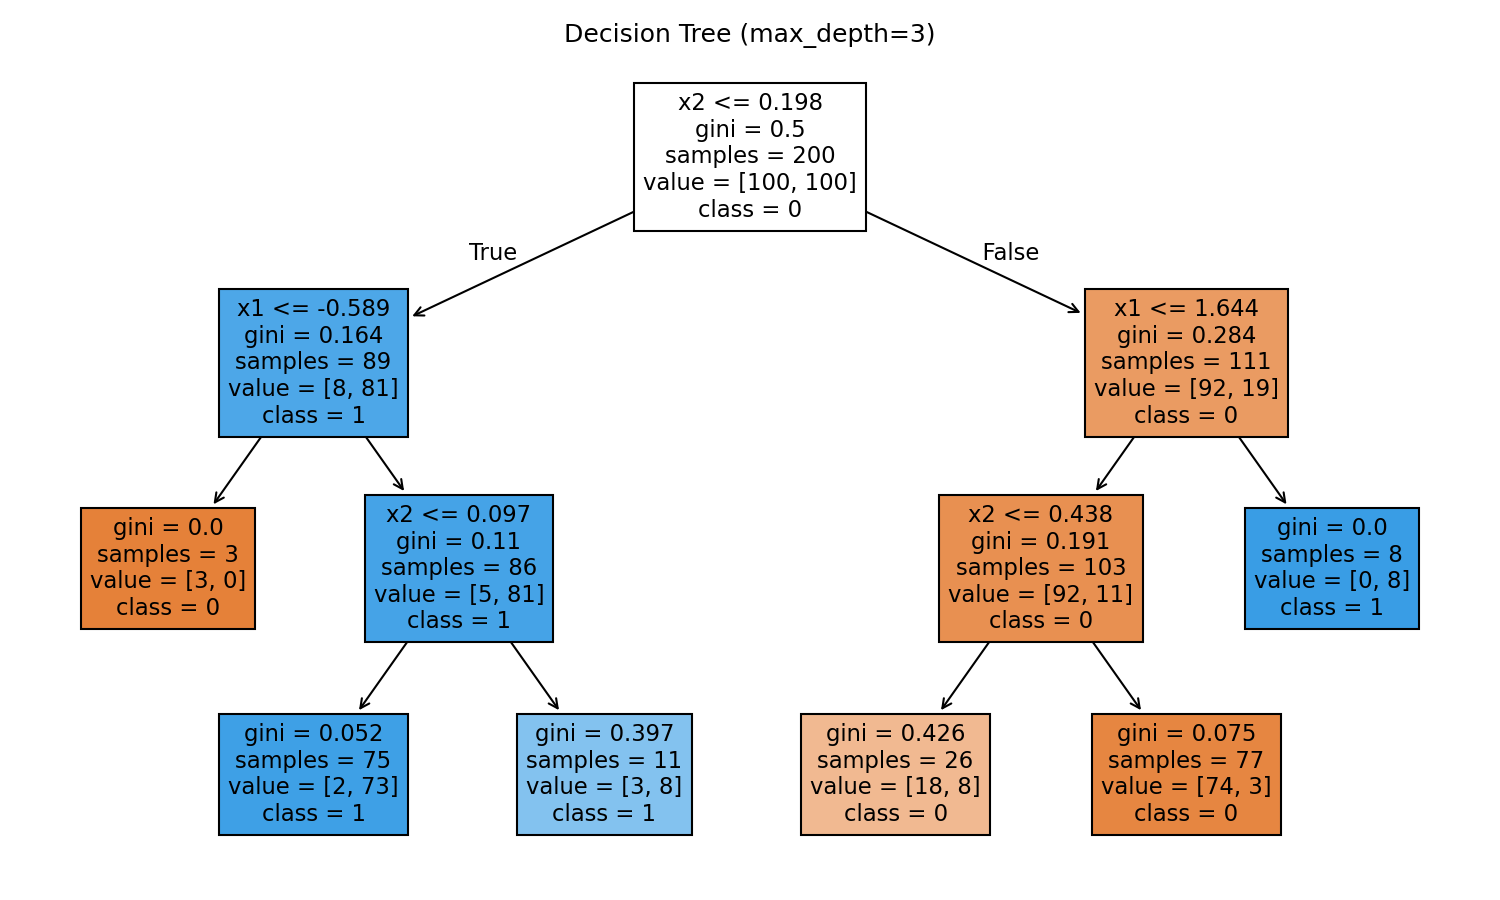
\includegraphics[width=0.95\linewidth]{dt_tree_plot.png}
  \caption{树结构可视化(max\_depth=3)。}
  \label{fig:treeplot_cn}
\end{figure}
\FloatBarrier

\section{总结}
决策树作为可解释且灵活的基线模型,在适当的正则化或与集成方法(随机森林、梯度提升)结合时,能在多种任务上取得具有竞争力的表现。

\end{document}
